
    First, the polyhedron needs to be written in standard form. In
    order to do so, we need to transform the constraints into equality
    constraints by introducing the slack variables $x_3$ and $x_4$ for
    the first and second equation, respectively. The constraints are
    then written as follows:
    \begin{align*}
        -x_1 + x_2 + x_3 \qquad & = 2, \\
        x_1 + x_2 \qquad + x_4 & = 4,\\
        x_1, x_2, x_3, x_4 & \geq 0.
    \end{align*}
    
    Given a feasible point of the polyhedron, it is possible to analyze if a direction is feasible by checking the following two conditions:
    \begin{itemize}
        \item $Ad = 0$, and
        \item $d_i \geq 0$ when $x_i = 0$,
    \end{itemize}
    where
    $$A \begin{pmatrix*}[r] -1 & 1 & 1 & 0 \\ 1 & 1 & 0 & 1 \end{pmatrix*}, x = \begin{pmatrix*}[r] x_1 \\ x_2 \\ x_3 \\ x_4 \end{pmatrix*}, d = \begin{pmatrix*}[r] d_1 \\ d_2 \\ d_3 \\ d_4 \end{pmatrix*}.$$
    
    
    Let's verify if these conditions are satisfied for the four cases.
    
    \begin{enumerate}

        \item $\tilde{x}_a = \begin{pmatrix*}[r] 0 \\ 2 \end{pmatrix*}$, $\tilde{d}_a = \begin{pmatrix*}[r] 1 \\ 0 \end{pmatrix*}.$ \\
        We first need to compute the values of the slack variables
        $x_3$ and $x_4$ and we obtain $x_3 = 0$ and $x_4 =
        2$. Therefore, we have
        \[
       x_a = \cvect{0 \\ 2 \\ 0 \\ 2},
       \]
       which is indeed a feasible point.

       We do the same for the vector $\tilde{x}_a+\tilde{d}_a = \left(\begin{array}{r} 1\\ 2 \end{array}\right)$.
       In standard form, it is $\left(\begin{array}{r} 1\\ 2 \\ 1 \\ 1 \end{array}\right)$.
       Therefore, the direction in standard form is
       \[
       d_a=\left(\begin{array}{r} 1\\ 2 \\ 1 \\ 1 \end{array}\right)-
       \left(\begin{array}{r} 0 \\ 2 \\ 0 \\ 2\end{array}\right) =
       \left(\begin{array}{r} 1\\ 0 \\ 1 \\ -1 \end{array}\right).
        \]


        In order to satisfy the first condition, we must have
        \begin{equation*}
        Ad_a = \begin{pmatrix*}[r] -1 & 1 & 1 & 0 \\ 1 & 1 & 0 & 1 \end{pmatrix*} \begin{pmatrix*}[r] 1 \\ 0 \\ 1 \\ -1 \end{pmatrix*} = \begin{pmatrix*}[r] 0 \\ 0 \end{pmatrix*},
        \end{equation*}
        which is verified. For the second condition, we look
        at the entries 1 and 3 of $d_a$, because $(x_a)_1=(x_a)_3=0$
        and the only zero entries. As
        $(d_a)_1=1$ and $(d_a)_3=1$, both entries of the direction
        are non negative and we conclude that the direction is feasible
        at the given point. 
        
%
%
%%%---part (b)---%%%
        \item $\tilde{x}_b = \begin{pmatrix*}[r] 0 \\ 2 \end{pmatrix*}$, $\tilde{d}_b = \begin{pmatrix*}[r] -1 \\ 0 \end{pmatrix*}.$ \\
        In this case, it is immediate to see that the direction is not
        feasible, as the second condition is not verified for the
        first entry: $(\tilde{d}_b)_1 = -1 < 0$ and $(\tilde{x}_b)_1 = 0$.
%
%
%%%---part (c)---%%%        
        \item $\tilde{x}_c = \begin{pmatrix*}[r] 2 \\ 2 \end{pmatrix*}$, $\tilde{d}_c = \begin{pmatrix*}[r] 0 \\ 2 \end{pmatrix*}.$ \\
        We compute the values of the slack variables: $x_3 = 2$, $x_4
        = 0$, so that
        \[
   {x}_c= \cvect{2 \\ 2 \\ 2 \\ 0}.
   \]
   We do the same for the vector $\tilde{x}_c+\tilde{d}_c = \left(\begin{array}{r} 2\\ 4 \end{array}\right)$.
   In standard form, it is $\left(\begin{array}{r} 2\\ 4 \\ 0 \\ -2 \end{array}\right)$.
   Therefore, the direction in standard form is
   \[ d_c = \left(\begin{array}{r} 2\\ 4 \\ 0 \\ -2 \end{array}\right)-
   \left(\begin{array}{r} 2 \\ 2 \\ 2 \\ 0\end{array}\right) =
   \left(\begin{array}{r} 0\\ 2 \\ -2 \\ -2 \end{array}\right).
   \]

   For the first condition to be satisfied, we must have
        \begin{equation*}
        Ad = \begin{pmatrix*}[r] -1 & 1 & 1 & 0 \\ 1 & 1 & 0 & 1 \end{pmatrix*} \begin{pmatrix*}[r] 0 \\ 2 \\ -2 \\ -2 \end{pmatrix*} = \begin{pmatrix*}[r] 0 \\ 0 \end{pmatrix*},
        \end{equation*}
        which is verified.
        For the second
        condition, we need to look at the entry 4 of $d_c$, as
        $({x}_c)_4=0$ is the only zero entry of $x_c$. As  $({d}_c)_4 = -2 < 0$, the second condition is not satisfied, and the  direction is not feasible at the given point.

%
%
%%%---part (d)---%%%     
        \item $\tilde{x}_d = \begin{pmatrix*}[r] 3 \\ 0 \end{pmatrix*}$, $\tilde{d}_d = \begin{pmatrix*}[r] 0 \\ 2 \end{pmatrix*}$ \\
        We compute the values of the slack variables: $x_3 = 5$, $x_4
        = 1$, so that
        \[
         {x}_d = \cvect{3 \\ 0 \\ 5 \\ 1}.
         \]
         We do the same for the vector $\tilde{x}_d+\tilde{d}_d =\left(\begin{array}{r} 3\\ 2 \end{array}\right)$.
         In standard form, it is $\left(\begin{array}{r} 3\\ 2 \\ 3 \\ -1 \end{array}\right)$.
         Therefore, the direction in standard form is
         \[d_d=\left(\begin{array}{r} 3\\ 2 \\ 3 \\ -1 \end{array}\right)-
         \left(\begin{array}{r} 3 \\ 0 \\ 5 \\ 1\end{array}\right) =
         \left(\begin{array}{r} 0\\ 2 \\ -2 \\ -2 \end{array}\right).
         \]
        For the first condition to be satisfied, we must have
        \begin{equation*}
        A{d}_d = \begin{pmatrix*}[r] -1 & 1 & 1 & 0 \\ 1 & 1 & 0 & 1 \end{pmatrix*} \begin{pmatrix*}[r] 0 \\ 2 \\ -2 \\ -2 \end{pmatrix*} = \begin{pmatrix*}[r] 0 \\ 0 \end{pmatrix*},
        \end{equation*}
        which is verified.
For the second condition, we need to look at the entry 2 of $d_d$, as
$x_2= 0$ is the only zero entry of $x$. As  $d_2 = 2 \geq 0$, the second condition is satisfied as well, and  the  direction is feasible at the given point.
    \end{enumerate}
    
    The following figure presents the four studied cases.
    \begin{center}
    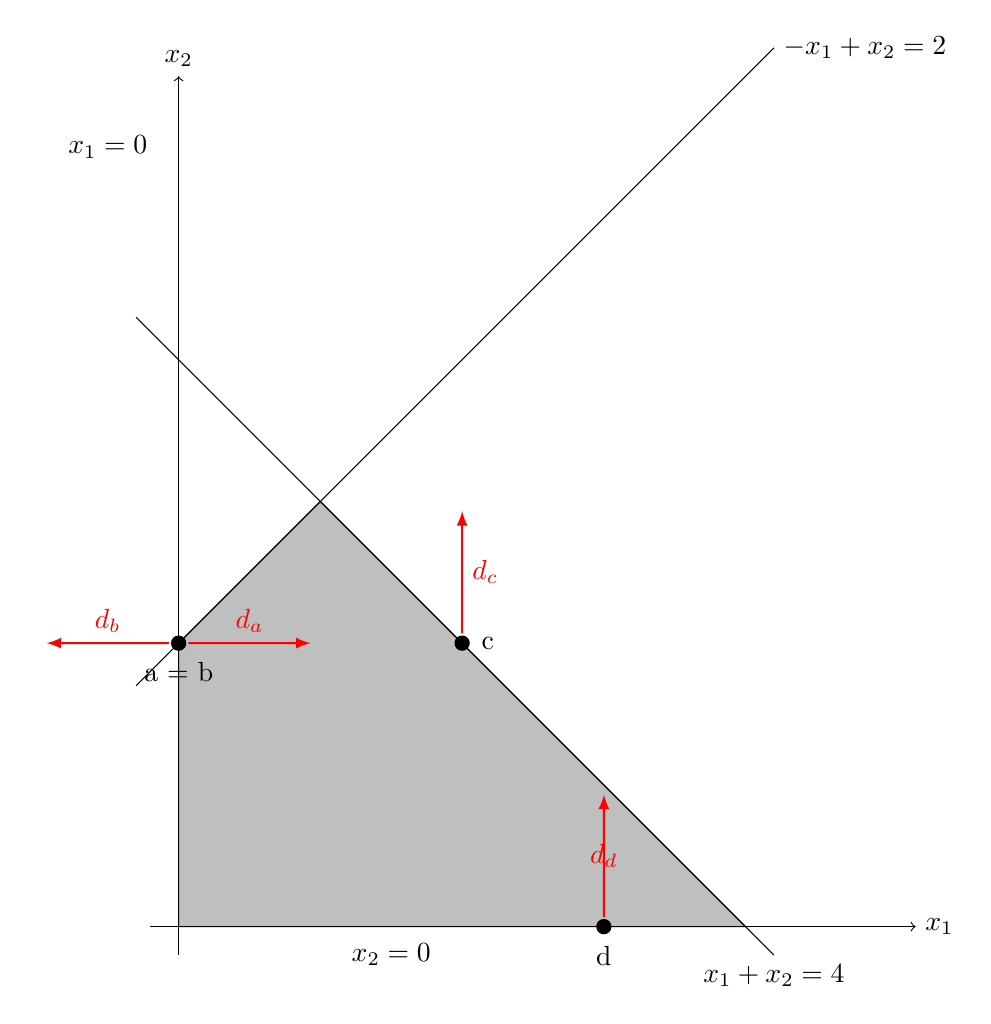
\begin{tikzpicture}[scale=1.8,domain=-0.3:4.2,range=-0.4:6]
      \draw[fill=lightgray]  (0,0) -- (0,2) -- (1,3) -- (4,0) -- cycle;
      \draw[->] (-0.2,0) -- (5.2,0) node[right] {$x_1$};
      \draw[->] (0,-0.2) -- (0,6) node[above] {$x_2$};
      \draw[color=black] plot (\x,\x+2) node[right] {$-x_1 + x_2 = 2$};
      \draw[color=black] plot (\x,4-\x) node[below] {$x_1 + x_2 = 4$};
      \node at (1.5,-0.2) {$x_2 = 0$};
      \node at (-0.5,5.5) {$x_1 = 0$};

      \node (A) at (0,2) [label=below:{a = b}] {};
      \draw[fill] (0,2) circle (0.05) ;
      \node (da) at (1,2) {} ;
      \draw[-latex,color=red,thick] (A) -- (da) node[midway,text=red,above] {$d_a$} ;

      \node (db) at (-1,2) {} ;
      \draw[-latex,color=red,thick] (A) -- (db) node[midway,text=red,above] {$d_b$} ;

      \node (C) at (2,2) [label=right:c] {};
      \draw[fill] (2,2) circle (0.05) ;
      \node (dc) at (2,3) {} ;
      \draw[-latex,color=red,thick] (C) -- (dc) node[midway,text=red,right] {$d_c$} ;
      
      \node (D) at (3,0) [label=below:d] {};
      \draw[fill] (3,0) circle (0.05) ;
      \node (dd) at (3,1) {} ;
      \draw[-latex,color=red,thick] (D) -- (dd) node[midway,text=red] {$d_d$} ;
      
      
    \end{tikzpicture}
    \end{center}

